\section{Introduction}

\subsection{3-D orbiter shape}
\begin{figure}[H]
 \centering
 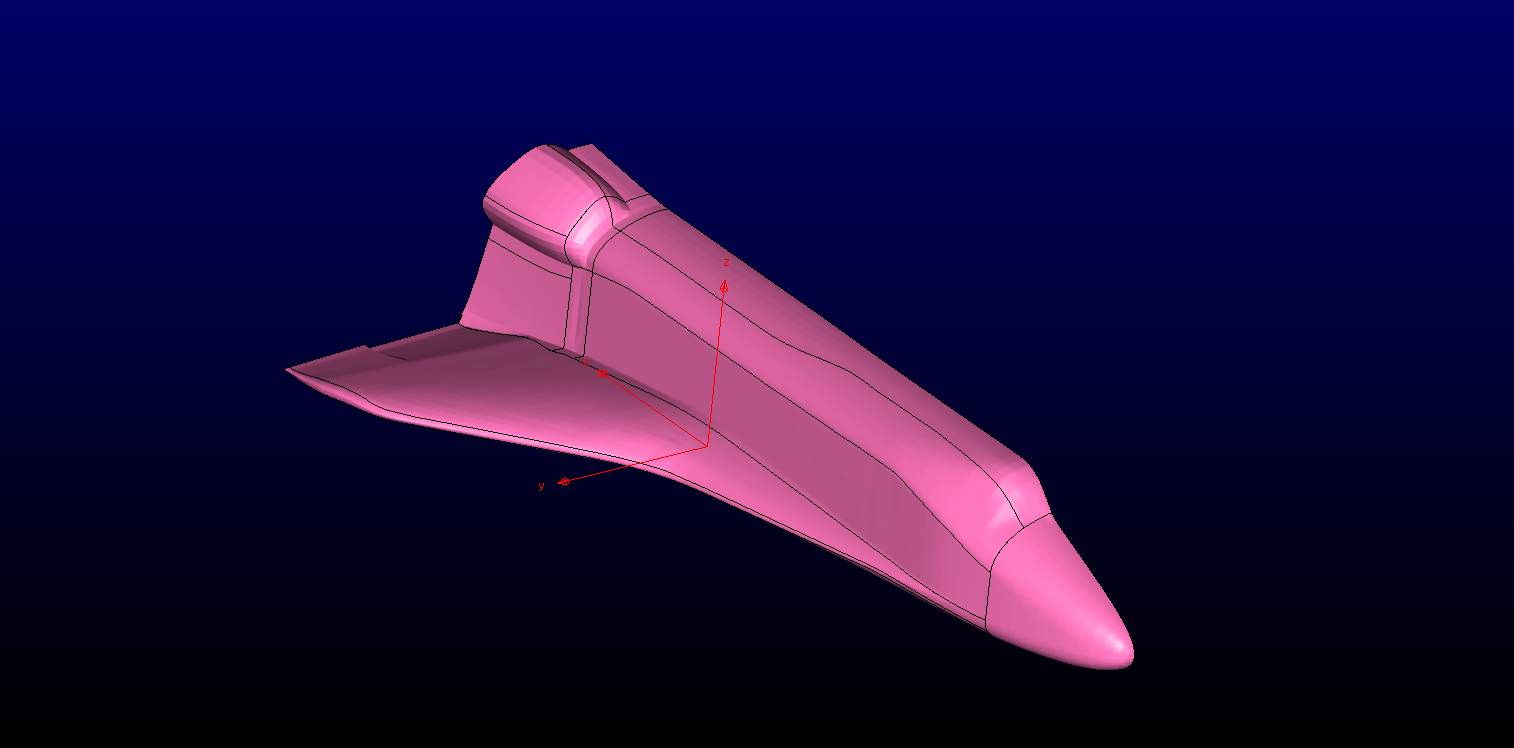
\includegraphics[width=\textwidth]{report_images/ss_image.png}
 \caption{3-D orbiter}
 \label{fig: ss_image}
\end{figure}

\subsection{Data from Published Texts}

\begin{figure}[ht!]
 \centering
 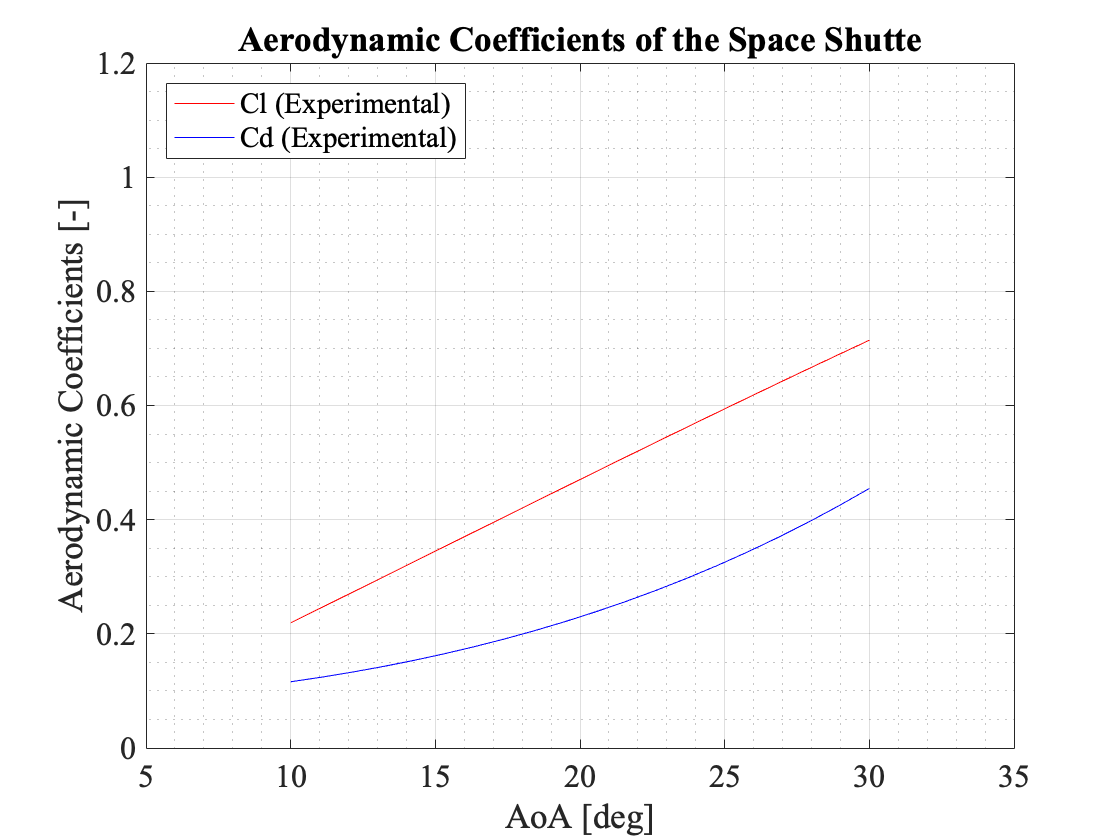
\includegraphics[width=0.7\textwidth]{matlab_images/aero_coeff_exp.png}
 \caption{Experimental models and predictions of $C_L$ \& $C_D$ for M = 3.8}
 \label{fig: coeff_exp}
\end{figure}

The equations used to plot the data in figure \ref{fig: coeff_exp} were from \cite{ss_prediction}

% REMEMBER TO INCLUDE THOSE THINGS WE SAID ABOUT THE VISCOSITY, TEMPERATURE AND STUFF LIKE PIECE-WISE POLYNOMIAL...

\begin{table}[H]
\centering
	\caption{Freestream conditions and expected stagnation conditions at wing/nose LE}
	\begin{tabular}{|c|c|} \hline
	Mach number           & 3.8 \\ \hline
	Post-shock mach number & 0.4407 \\ \hline
	Pressure $p$ \footnote{test}	& 1090.16 Pa \\ \hline
	Temperature $T$ 	& 227.13 K	\\ \hline
	Density $\rho$ 	& 0.0167 kg $\cdot$ m$^{-3}$ \\ \hline
	$\nicefrac{p_2}{p_1}$ at M=3.8 & 16.68 \\ \hline
	$\nicefrac{T_2}{T_1}$ at M=3.8 & 3.743 \\ \hline
	Isentropic $\nicefrac{p_o}{p}$ at M=0.44 & 1.142 \\ \hline
	Isentropic $\nicefrac{T_o}{T}$ at M=0.44 & 1.035 \\ \hline
	Stagnation pressure		& 20765.98 Pa ($p \cdot \nicefrac{p_2}{p_1} \cdot \nicefrac{p_o}{p}$) \\ \hline
	Stagnation temperature	& 883.303 K ($T \cdot \nicefrac{T_2}{T_1} \cdot \nicefrac{T_o}{T}$) \\ \hline
	\end{tabular}
\end{table}
\noindent$p, T, \rho$: at 100,000 ft from 1976 Digital Dutch Standard Atmospheric Calculator \\ \indent (URL: https://www.digitaldutch.com/atmoscalc/) \\
\noindent Isentropic relations and pressure/temp discontinuity across shock: From appendix A of Modern Compressible \\ \indent Flow by J.D. Anderson \cite{anderson_comp_flow}.
